\documentclass[10pt]{beamer}
\usetheme{jambro}

\title[]{Macroeconomia I - Curva IS e Demanda Agregada}
\author[]{Paulo Victor da Fonseca}
\date{}

\hypersetup{
    colorlinks = true,
    urlcolor = teal,
    linkcolor = teal    
}
\usepackage[portuguese]{babel}
\usepackage{subfig}
\usepackage{emoji}
\usepackage{hyperref}

\begin{document}

\begin{frame}[plain]
    \titlepage{
        \begin{center}
            \begin{minipage}{0.8\textwidth}
                \centering
            \end{minipage}
        \end{center}}
\end{frame}

\begin{frame}{Sumário}
    \tableofcontents
\end{frame}

\section{Introdução}
\begin{frame}{Introdução}
    \begin{itemize}
        \item Nas aulas anteriores estudamos a determinação do equilíbrio no mercado de bens e serviços.
        \bigskip
        \item Nosso objetivo, agora, é iniciar os estudos dos mercados financeiros e como as operações do Banco Central afetam as taxas de juros.
        \bigskip
        \item Os mercados financeiros envolvem uma rede intrincada de instituições (bancos, fundos do mercado monetário, fundos mútuos, fundos de investimento e fundos \emph{hedge}).
        \bigskip
        \item As transações envolvem títulos, ações e outros créditos financeiros como \emph{swaps} e opções.
        \bigskip
        \item Além disso, existe um conjunto enorme de taxas de juros: taxas de juros de muitos tipos diferentes de títulos do governo, diversos títulos corporativos, de títulos de curto prazo, de títulos de longo prazo, etc.
    \end{itemize}
\end{frame}

\begin{frame}{Introdução}
    \begin{itemize}
        \item Os mercados financeiros desempenham um papel fundamental na economia, determinam os custos dos fundos para empresas, famílias e governo e, consequentemente, afetam suas decisões de gastos.
        \bigskip
        \item Como nosso objetivo é estudar o papel do Banco Central em afetar as taxas de juros, consideraremos um modelo super simplificado de uma economia com apenas dois ativos: moeda (que não paga juros) e títulos (que pagam).
        \bigskip
        \item Isso nos permitirá entender como a taxa de juros dos títulos é determinada e o papel do Banco Central nesta determinação.
    \end{itemize}
\end{frame}

\section{Demanda por moeda}
\subsection{Moeda, renda e riqueza}
\begin{frame}{Moeda, renda e riqueza}
    \begin{itemize}
        \item \textcolor{blue}{Moeda:} é o que se pode usar para pagar transações e pode ser papel-moeda ou depósitos à vista em bancos.
        \bigskip
        \item \textcolor{blue}{Renda:} é o que se ganha com o trabalho mais o que se recebe em juros e dividendos. A renda é uma variável de \textbf{fluxo}, ou seja, algo expresso em unidades de tempo (renda mensal, renda anual, etc.).
        \bigskip
        \item \textcolor{blue}{Riqueza financeira:} ou simplesmente riqueza, é o valor de todos os ativos financeiros menos todos os passivos financeiros. A riqueza é uma variável de \textbf{estoque}, ou seja, é o valor da riqueza em dado instante do tempo.
        \bigskip
        \item Em dado instante do tempo não se pode alterar o montante total da riqueza financeira. Só se pode fazer isso ao longo do tempo, à medida que se poupa e despoupa, ou à medida que os valores dos ativos e passivos variam.
    \end{itemize}
\end{frame}

\begin{frame}{Moeda, renda e riqueza}
\begin{itemize}
    \item É possível, no entanto, mudarmos a composição da riqueza em um dado instante do tempo. Por exemplo, podemos pagar parte da hipoteca emitindo um cheque da conta-corrente. Isto leva a uma diminuição dos passivos (hipoteca menor) e a uma diminuição equivalente dos ativos (um saldo menor em conta-corrente). Enquanto mantem a riqueza inalterada.
    \bigskip
    \item Os ativos financeiros que podem ser usados diretamente para comprar bens são chamados de \emph{moeda} e incluem o papel-moeda e os depósitos à vista, ou seja, depósitos contra os quais se pode emitir cheques. A moeda também é uma variável de estoque.
\end{itemize}
\end{frame}

\subsection{Demanda por moeda}
\begin{frame}{Demanda por moeda}
    \begin{itemize}
        \item Suponha que um indivíduo, por ter poupado regularmente parte de sua renda no passado, possua uma riqueza financeira atual de \$50.000.
        \bigskip
        \item Este indivíduo pode continuar poupando no futuro e, com isso, aumentar sua riqueza. No entanto, seu valor atual já está determinado.
        \bigskip
        \item Por hipótese, vamos supor que este indivíduo pode decidir como alocar sua riqueza financeira somente entre dois tipos de ativos - moeda e títulos.
    \end{itemize}
\end{frame}

\begin{frame}{Demanda por moeda}
    \begin{itemize}
        \item A \textcolor{blue}{moeda}, que pode ser usada para transações, não paga juros. Existem dois tipos de moeda: \textbf{papel-moeda} - moedas e notas em espécie - e \textbf{depósitos à vista} - os depósitos bancários sobre os quais é possível emitir cheques ou utilizar o cartão de débito.
        \bigskip
        \item Os \textcolor{blue}{títulos}, por sua vez, pagam uma taxa de juros positiva, $i$, mas não podem ser usados em transações. Cabe ressaltar que, no mundo real, há muitos tipos de títulos, cada qual associado a uma taxa de juros específica. Por enquanto, vamos ignorar este aspecto da realidade e considerar que haja apenas um tipo de título que pague uma taxa de juros $i$.
    \end{itemize}
\end{frame}

\begin{frame}{Demanda por moeda}
    \begin{itemize}
        \item Vamos supor que a compra e venda de títulos implique algum custo - e.g., taxa de corretagem.
        \bigskip
        \item Quanto de sua riqueza financeira de \$50.000 este indivíduo deveria reter em moeda e quanto em títulos?
        \bigskip
        \begin{enumerate}
            \item Manter toda a riqueza sob forma de moeda é conveniente. Mas isto implica em não receber nenhuma renda em juros.
            \bigskip
            \item Por outro lado, manter toda a riqueza sob forma de títulos é bastante inconveniente, mesmo que este indivíduo receba juros sobre o montante total. Isto porque deverá contatar seu corretor frequentemente para qualquer transação que precisar fazer no dia a dia.
        \end{enumerate}
    \end{itemize}
\end{frame}

\begin{frame}{Demanda por moeda}
    \begin{itemize}
        \item Portanto, este indivíduo deveria alocar sua riqueza tanto em moeda quanto em títulos.
        \bigskip
        \item Para respondermos em qual proporção, devemos considerar as seguintes duas variáveis:
        \bigskip
        \begin{enumerate}
            \item \textcolor{blue}{Nível de transações:} o indivíduo desejará ter moeda suficiente à disposição para evitar a venda frequente de títulos em troca de moeda.
            \bigskip
            \item \textcolor{blue}{Taxa de juros dos títulos:} o único motivo para reter parte da riqueza em títulos é que eles pagam juros. Quanto mais alta a taxa de juros, mais disposto este indivíduo estará a enfrentar o trabalho e custos associados à compra e venda de títulos.
        \end{enumerate}
    \end{itemize}
\end{frame}

\subsection{Derivação da demanda por moeda}
\begin{frame}{Derivação da demanda por moeda}
\begin{itemize}
    \item Seja o montante de moeda que as pessoas desejam reter - sua \textcolor{blue}{demanda por moeda} - dado por $M^d$. A demanda por moeda na economia é a soma de todas as demandas por moeda individuais.
    \bigskip
    \item Portanto, ela depende do nível total de transações na economia e da taxa de juros.
    \bigskip
    \item A mensuração do nível total de transações na economia é difícil de ser obtida. Mas podemos usar a renda agregada nominal como uma \emph{proxy}.
    \bigskip
    \item Portanto, a relação entre a demanda por moeda, renda nominal e taxa de juros pode ser descrita pela seguinte equação:
    \begin{equation}
        M^d = \$Y L(i), \qquad L'(i) < 0.
        \label{eq1}
    \end{equation}
    em que $\$ Y$ representa a renda nominal.
\end{itemize}
\end{frame}

\begin{frame}{Derivação da demanda por moeda}
    \begin{itemize}
        \item A equação (\ref{eq1}) nos diz que a demanda por moeda, $M^d$, é igual à renda nominal, $\$Y$, multiplicada por uma função da taxa de juros, $i$, representada por $L(i)$:
        \bigskip
        \begin{enumerate}
            \item A demanda por moeda aumenta em proporção à renda nominal. Se a renda nominal dobra, a demanda por moeda também dobra.
            \bigskip
            \item A demanda por moeda depende negativamente da taxa de juros, ou seja, um aumento na taxa de juros diminui a demanda por moeda.
        \end{enumerate}
    \end{itemize}
\end{frame}

\begin{frame}{Derivação da demanda por moeda}
    \begin{figure}
        \centering
        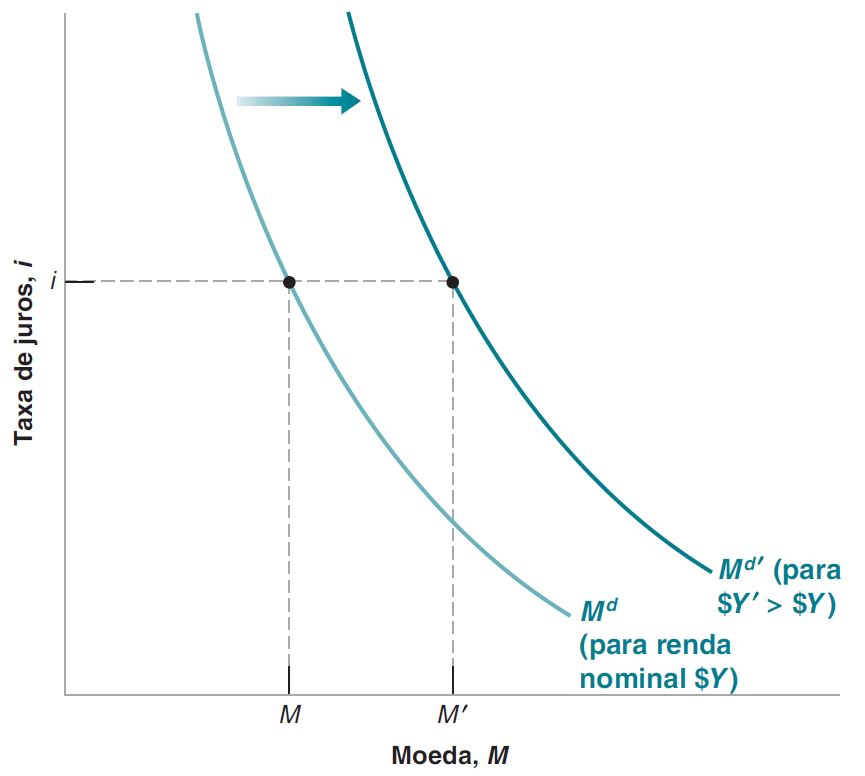
\includegraphics[width=0.7\textwidth]{./figures/aula072_fig1.JPG}
        \caption{Demanda por moeda. Fonte: Blanchard (2017).}
        \label{fig1}
    \end{figure}
\end{frame}

\section{Determinação da taxa de juros: parte I}
\subsection{Determinação da taxa de juros}
\begin{frame}{Demanda por moeda, oferta de moeda e taxa de juros de equilíbrio}
    \begin{itemize}
        \item Como dito anteriormente, existem dois tipos de moeda: depósitos à vista (ofertados pelos bancos) e papel-moeda (ofertada pelo Banco Central).
        \bigskip
        \item Por simplicidade, consideraremos, inicialmente, que a oferta de moeda é dada apenas pelo papel-moeda.
        \bigskip
        \item Vamos supor que o Banco Central decida ofertar um montante de moeda igual a $M$, de modo que:
        \[
        M^s = M.
        \]
    \end{itemize}
\end{frame}

\begin{frame}{Demanda por moeda, oferta de moeda e taxa de juros de equilíbrio}
\begin{itemize}
    \item O equilíbrio nos mercados financeiros requer que a oferta de moeda seja igual à demanda por moeda. Portanto, temos a seguinte condição de equilíbrio:
    \begin{equation}
        M = \$Y L(i).
        \label{eq3}
    \end{equation}
    \bigskip
    \item A taxa de juros $i$ deve ser tal que, dada a renda nominal, as pessoas estejam dispostas a ter um montante de moeda igual à oferta de moeda existente $M$.
\end{itemize}
\end{frame}

\begin{frame}{Demanda por moeda, oferta de moeda e taxa de juros de equilíbrio}
\begin{figure}
    \centering
    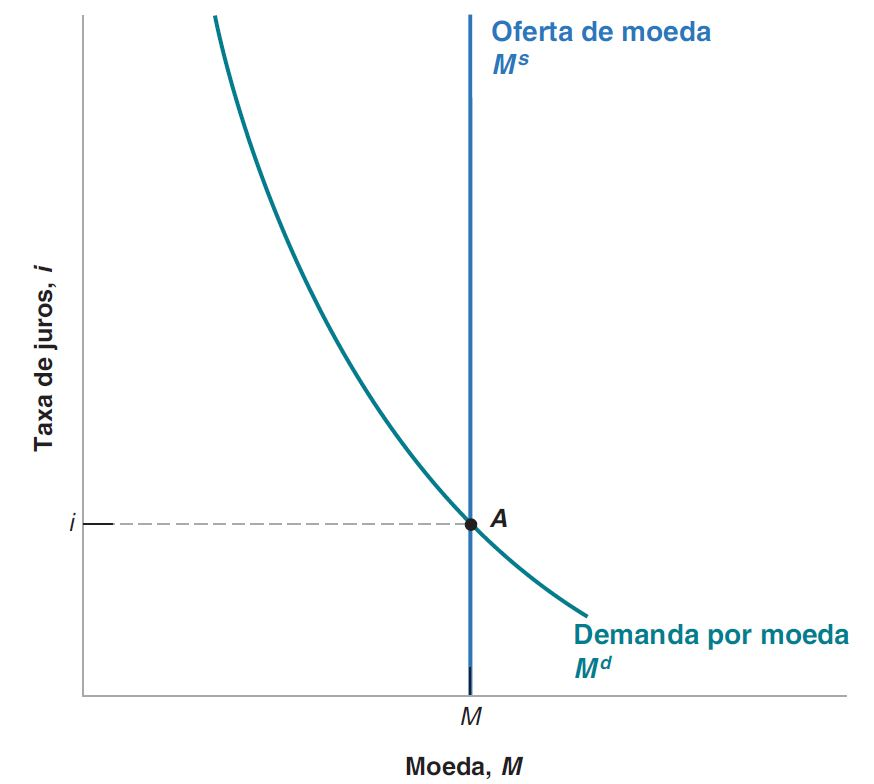
\includegraphics[width=0.6\textwidth]{./figures/aula072_fig2.JPG}
    \caption{Determinação da taxa de juros. Fonte: Blanchard (2017).}
    \label{fig2}
\end{figure}
\end{frame}

\begin{frame}{Efeitos de um aumento na renda nominal sobre a taxa de juros}
    \begin{figure}
        \centering
        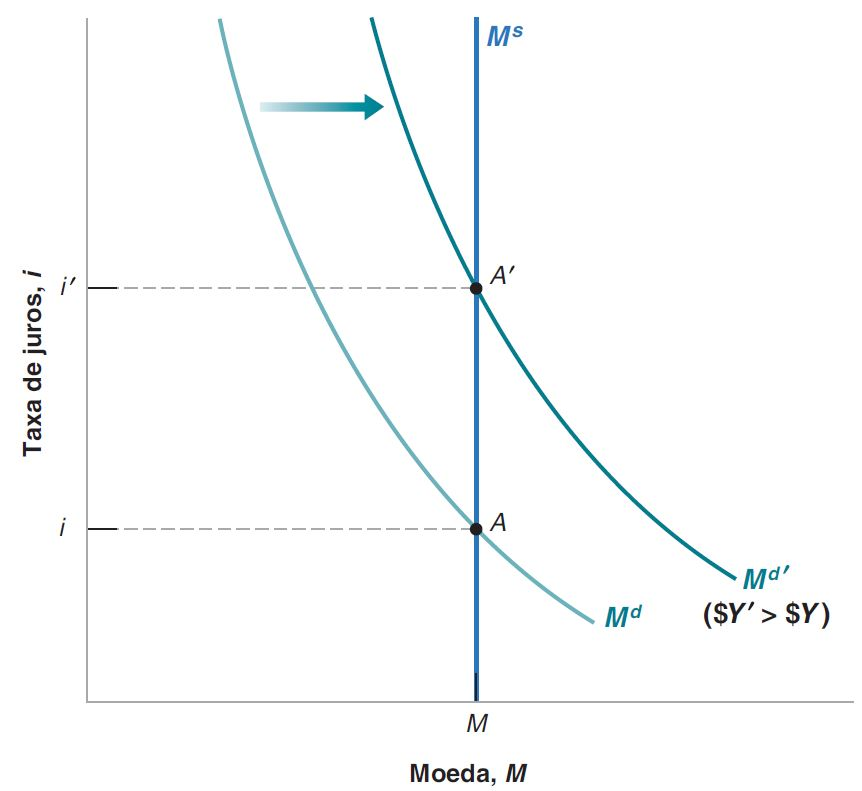
\includegraphics[width=0.55\textwidth]{./figures/aula072_fig3.JPG}
        \caption{Efeitos de um aumento na renda nominal sobre a taxa de juros. Fonte: Blanchard (2017).}
        \label{fig3}
    \end{figure}
\end{frame}

\begin{frame}{Efeitos de um aumento na renda nominal sobre a taxa de juros}
%\begin{itemize}
%    \item Um aumento da renda nominal de $\$Y$ para $\$ Y'$ aumenta o nível de transações, que aumenta a demanda por moeda a qualquer taxa de juros.
%    \bigskip
%    \item A curva de demanda por moeda se desloca para a direita, de $M^d$ para $M^d'$.
%    \bigskip
%    \item O equilíbrio se move para cima, de $A$ para $A'$, e a taxa de juros de equilíbrio aumenta de $i$ para $i^'$.
%    \bigskip
%    \item Portanto, para uma dada oferta de moeda exógena, um aumento da renda nominal leva a um aumento da taxa de juros de equilíbrio.
%    \bigskip
%    \item À taxa de juros inicial, a demanda por moeda excede a oferta. Logo, um aumento da taxa de juros é necessário para diminuir o montante de moeda que as pessoas desejam reter e para restabelecer o equilíbrio.
%\end{itemize}
%\end{frame}

\begin{frame}{Efeitos de um aumento da oferta de moeda sobre a taxa de juros}
    \begin{figure}
        \centering
        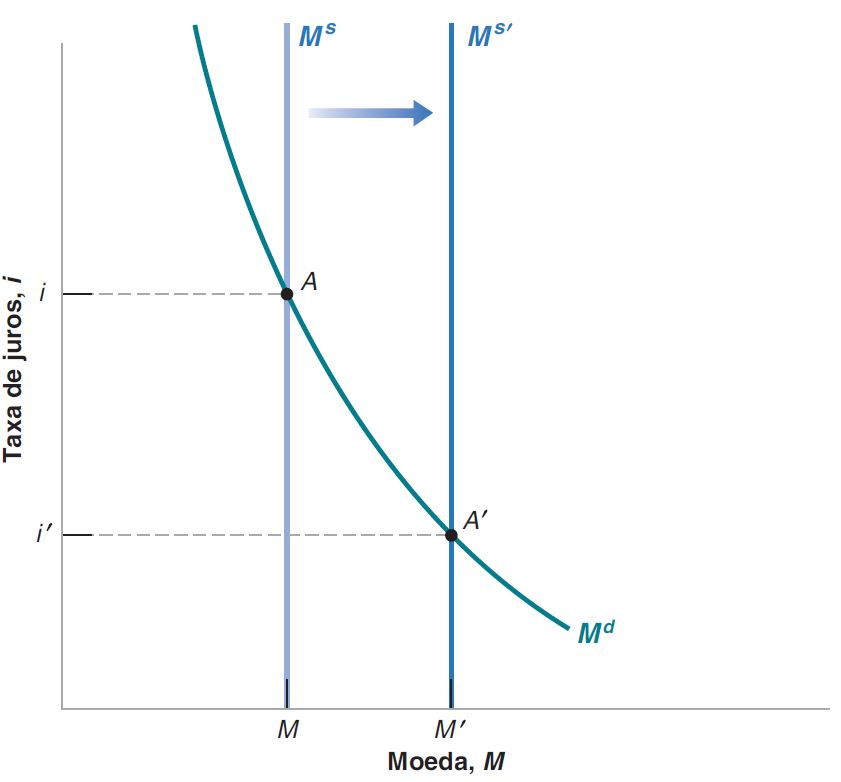
\includegraphics[width=0.5\textwidth]{./figures/aula072_fig4.JPG}
        \caption{Efeitos de um aumento da oferta de moeda sobre a taxa de juros. Fonte: Blanchard (2017).}
        \label{fig4}
    \end{figure}
\end{frame}

\begin{frame}{Efeitos de um aumento da oferta de moeda sobre a taxa de juros}
\begin{itemize}
    \item Um aumento da oferta de moeda leva a um deslocamento da curva de oferta de moeda para a direita, de $M^s$ para $M^s'$.
    \bigskip
    \item O equilíbrio se move para baixo, de $A$ para $A'$, e a taxa de juros de equilíbrio diminui de $i$ para $i'$.
    \bigskip
    \item Portanto, um aumento da oferta de moeda pelo Banco Central leva a uma redução da taxa de juros.
    \bigskip
    \item A redução da taxa de juros aumenta a demanda por moeda de modo que ela seja igual à maior oferta de moeda.
\end{itemize}
\end{frame}

\subsection{Política monetária e operações de mercado aberto}
\begin{frame}{Operações de mercado aberto}
\begin{itemize}
    \item Nas economias modernas, o modo pelo qual a autoridade monetária (Banco Central) altera a oferta de moeda consiste na compra e venda de títulos no mercado de títulos.
    \bigskip
    \item Se um BC deseja aumentar o montante de moeda em circulação na economia, compra títulos e paga por eles por meio da criação de moeda.
    \bigskip
    \item Se deseja diminuir o montante de moeda, vende títulos e retira de circulação a moeda que recebe em troca desses títulos.
    \bigskip
    \item Essas ações são chamadas \textcolor{blue}{operações de mercado aberto}, porque ocorrem no ``mercado aberto'' de títulos.
\end{itemize}    
\end{frame}

\begin{frame}{O balancete do Banco Central}
    \begin{itemize}
        \item Para compreender as operações de mercado aberto, é útil entendermos o balancete patrimonial do Banco Central.
        \bigskip
        \item Os \textcolor{blue}{ativos} do BC são a soma de títulos que ele retém em sua carteira.
        \bigskip
        \item O \textcolor{blue}{passivo} é o estoque de moeda em circulação na economia.
        \bigskip
        \item As operações de mercado aberto levam a mudanças iguais do ativo e do passivo.
        \bigskip
        \item Se o BC compra (vende), por exemplo, $\$ 1$ milhão em títulos, o montante de títulos em sua carteira aumenta (diminui) em $\$ 1$ milhão e, da mesma forma, o estoque de moeda na economia também aumenta (diminui) na mesma proporção. Esta operação é chamada \textcolor{blue}{operação de mercado aberto expansionista (contracionista)}, porque o BC expande (contrai) a oferta de moeda.
    \end{itemize}
\end{frame}

\begin{frame}{O balancete do Banco Central}
\begin{figure}
    \centering
    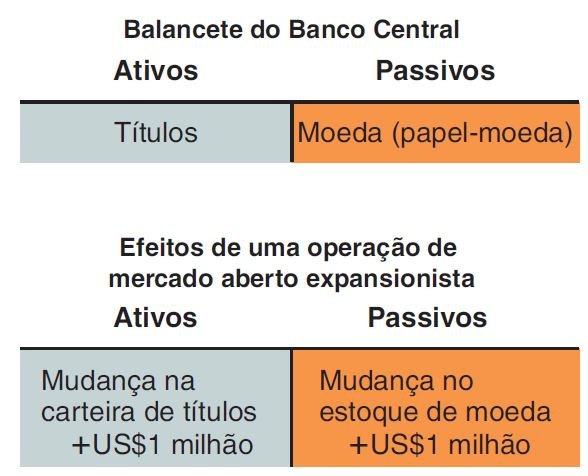
\includegraphics[width=0.7\textwidth]{./figures/aula072_fig5.JPG}
    \caption{Balancete patrimonial do Banco Central. Fonte: Blanchard (2017).}
    \label{fig5}
\end{figure}
\end{frame}

\begin{frame}{Preço $\times$ rendimento de títulos}
    \begin{itemize}
        \item Até aqui nos concentramos na taxa de juros dos títulos. Na realidade, o que é determinado nos mercados de títulos não são as taxas de juros, mas os \textcolor{blue}{preços} dos títulos.
        \bigskip
        \item No entanto, os preços de títulos e suas taxas de juros estão diretamente relacionados.
        \bigskip
        \item Suponhamos que os títulos em nossa economia sejam de um ano - títulos que prometem pagar uma certa quantidade de moeda daqui um ano.
        \bigskip
        \item Nos EUA, títulos emitidos pelo governo com promessa de pagamento em um ano ou menos são chamados de \textbf{letras do Tesouro} ou, simplesmente, \textbf{T-bills}.
    \end{itemize}
\end{frame}

\begin{frame}{Preço $\times$ rendimento de títulos}
\begin{itemize}
    \item Suponha um título que promete pagar $\$ 100$ daqui a um ano. Seja o preço deste título hoje igual a $\$ P_B$. Se um indivíduo comprar este título hoje e o mantiver por um ano, a taxa de retorno da posse do título por um ano será igual a $(\$ 100 - \$P_B)/\$ P_B$. Portanto, a taxa de juros do título é dada por:
    \[
    i = \frac{\$ 100 - \$P_B}{\$P_B}.
    \]
    Ou seja, \textbf{quanto maior for o preço do título, menor será a taxa de juros}.
    \bigskip
    \item Se soubermos a taxa de juros, podemos descobrir o preço do título:
    \[
    \$P_B = \frac{\$100}{1 + i}.
    \]
    Se a taxa de juros é positiva, o preço do título é menor que o pagamento final. \textbf{Quanto maior a taxa de juros, menor o preço atual do título}.
\end{itemize}
\end{frame}

\begin{frame}{Operações de mercado aberto}
    \begin{itemize}
        \item Portanto, ao realizar uma operação de mercado aberta expansionista, o BC compra títulos no mercado de títulos e paga por eles por meio da criação de moeda.
        \bigskip
        \item À medida que o BC compra títulos, a demanda por títulos cresce, aumentando seus preços.
        \bigskip
        \item Reciprocamente, a taxa de juros dos títulos cai.
        \bigskip
        \item Note que, ao comprar títulos em troca da moeda que criou, o Banco Central expandiu a base monetária (aumentou a oferta de dinheiro).
        \bigskip
        \item Portanto, ao comprar ou vender títulos em troca de moeda, o Banco Central afeta o preço dos títulos e, consequentemente, a taxa de juros sobre os títulos.
    \end{itemize}
\end{frame}

\section{Resumo}
\begin{frame}
    \begin{itemize}
        \item A taxa de juros é determinada pela igualdade entre oferta de moeda e demanda por moeda.
        \bigskip
        \item Ao alterar a oferta de moeda, o Banco Central pode afetar a taxa de juros.
        \bigskip
        \item O Banco Central altera a oferta de moeda por meio de operações de mercado aberto, que são compras ou vendas de títulos em troca de moeda.
        \bigskip
        \item As operações de mercado aberto nas quais o BC aumenta a oferta de moeda por meio da compra de títulos levam a um aumento nos preços dos títulos e a uma diminuição na taxa de juros. A curva de oferta de moeda é deslocada para direita.
        \bigskip
        \item As operações de mercado aberto nas quais o BC diminui a oferta de moeda por meio da venda de títulos levam a uma diminuição no preço dos títulos e a um aumento na taxa de juros. A curva de oferta de moeda é deslocada para esquerda.
    \end{itemize}
\end{frame}

\begin{frame}{\emoji{books} Bibliografia}
    \begin{itemize}
        \item BLANCHARD, O. Macroeconomia. 7.ed. São Paulo: Pearson Education do Brasil, 2017\medskip        
        \item CARLIN, W.; SOSKICE, D. Macroeconomics: Institutions, instability, and the financial system. Oxford, UK: Oxford University Press, 2015\medskip
        \item DORNBUSCH, R.; FISCHER, S.; STARTZ, R. Macroeconomia. 11.ed. Porto Alegre: AMGH, 2013. Disponível em: \href{https://app.minhabiblioteca.com.br/books/9788580551853}{app.minhabiblioteca.com.br/books/9788580551853}\medskip
        \item MISHKIN, F.S. The economics of money, banking, and financial markets. 11.ed. Pearson Education Limited, England, 2016.
    \end{itemize}
\end{frame}
\end{document}